\documentclass[11pt]{article}
\usepackage{amsmath, amssymb, amsfonts,  graphicx, enumerate, float, wrapfig}
\usepackage[margin=0.5in]{geometry}
\graphicspath{{./}}
\newcommand*{\vs}{\vspace{1cm}}
\newcommand*{\next}{\noindent}
\newcommand*{\set}{\setcounter{equation}{0}}


\title{Notes - 3.9 Differentials}
\author{Juan J. Moreno Santos}
\date{November 2023}

\begin{document}
\maketitle

\section{Warm-up}
1. If $f(x)=x^5-1$, $f^{-1}$ is:
\begin{align}
    f^{-1}(x)&=\sqrt[5]{x+1}
\end{align}
2. $\frac{d}{dx}(x^2-3xy+y^2=-1)$ at $(1, 1)$:
\begin{align}
    \set
    f(x)&=x^2-3xy+y^3=-2\\
    \frac{dy}{dx}&=3xdx-3ydx+(-3xdy)+2ydy=0\\
    &2ydy-3xdy=3ydx-2xdx\\
    &dy(2y-3x)=dx(3y-2x)\\
    &\frac{dy}{dx}=\frac{3y-2x}{2y-3x}=\frac{3(1)-2(1)}{2(1)-3(1)}=-1
\end{align}

\section[scale=0.5]{3.9 Differentials}
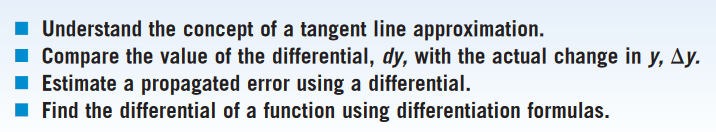
\includegraphics{LO.png}\\
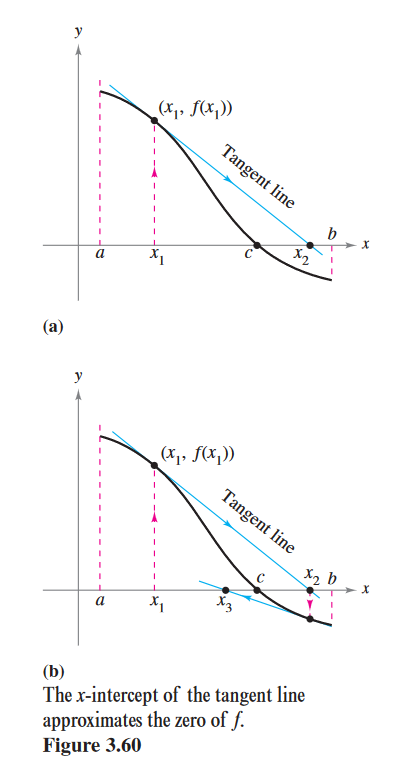
\includegraphics{3.8.png}
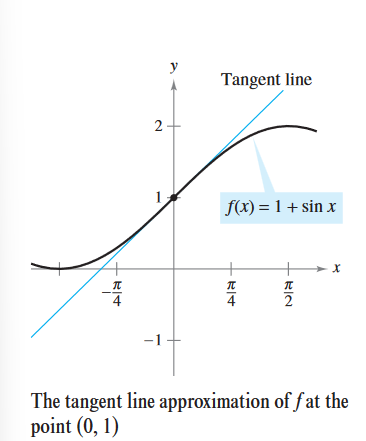
\includegraphics{3.9.png}\\
We are familiar with the point-slope form of a function:
\[(y-y_1)=m(x-x_1)\]
The euqation for the tangent line at the point $(c, f(c))$ is given by:
\[y-f(c)=f'(c)(x-c)\]
\[y=f(c)+f'(c)(x-c)\]
It has the same format as the point-slope form of a function.\\

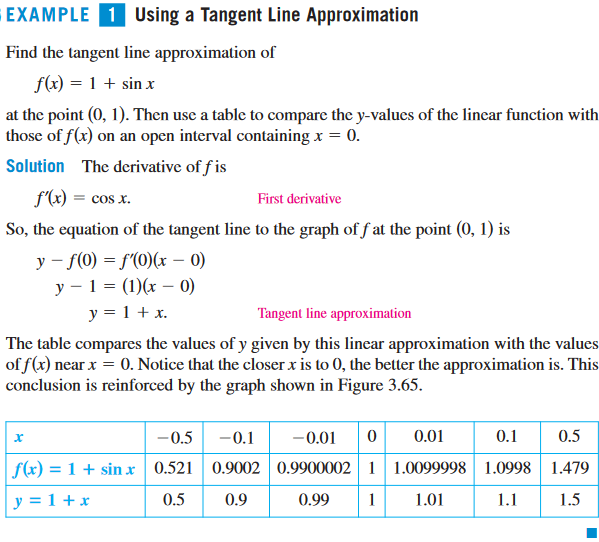
\includegraphics{ex1.png}\\
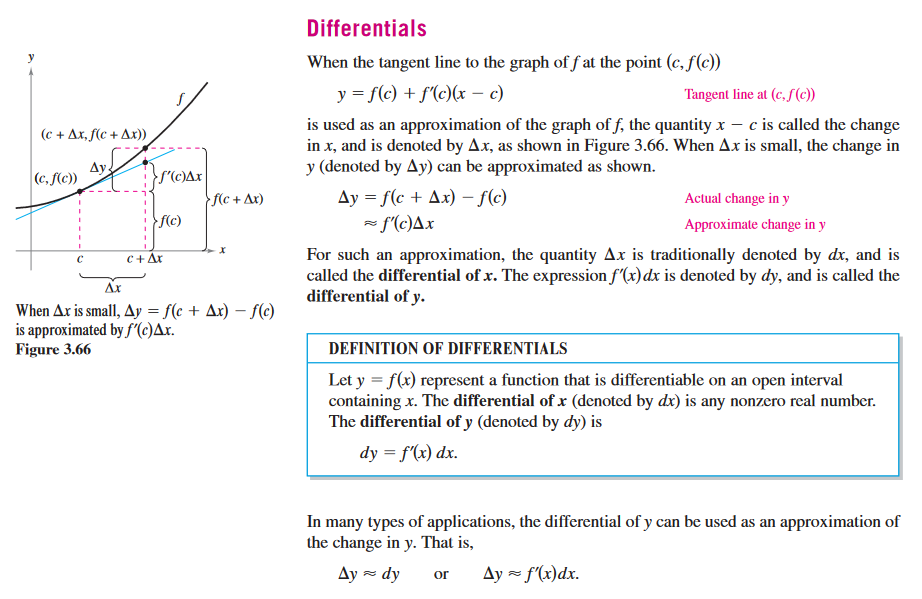
\includegraphics[scale=0.75]{diff.png}\\
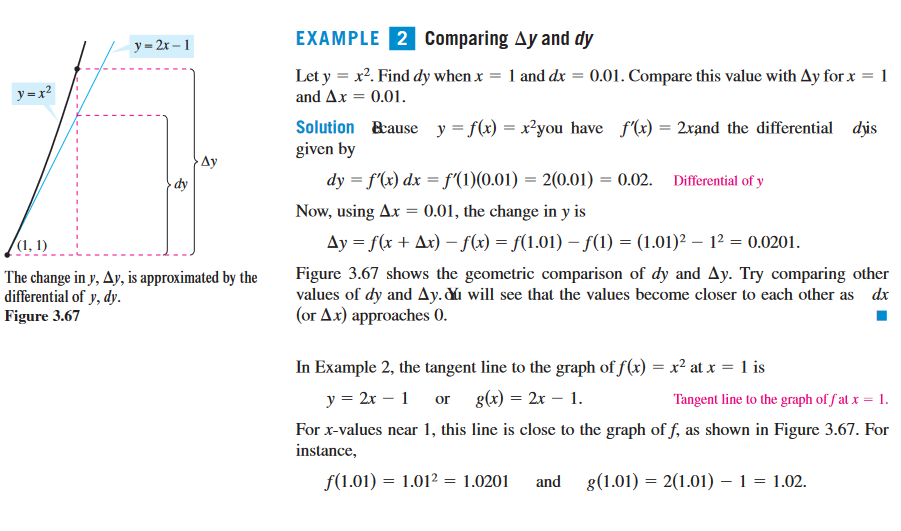
\includegraphics[scale=0.75]{ex2}
In other words,
\begin{align}
    \set
    y&=x^2\\
    dy&=f'(x)dx=2xdx=2(1)(0.01)\\
    &=0.02\\
\end{align}
For the tangent line:
\begin{align}
    y&=f(c)+f'(c)(x-c)\\
    &=1-2(x-1)\\
    &=2x-1
\end{align}
Therefore,
\begin{align}
    \Delta y&=f(x+\Delta x)-f(x)\\
    &=f(1+0.1)-f(1)\\
    &=(1.01)^2-(1)^2\\
    &=0.201
\end{align}
Comparing to equation 4, we can confirm that $\Delta y \approx dy$

\section{Error propagation}
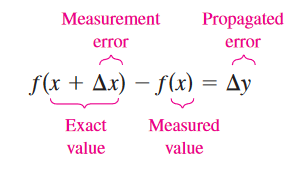
\includegraphics{prop.png}\\
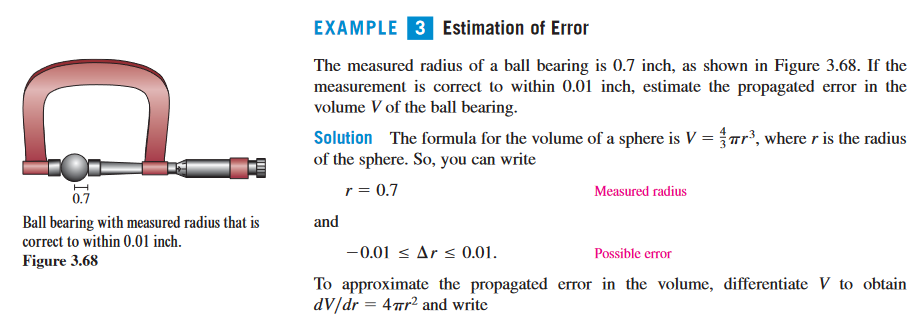
\includegraphics[scale=0.75]{ex3.png}
\begin{align}
    \set
    V&=\frac{4}{3}\pi r^3\\
    dV&=4\pi r^2dr\\
    &=4\pi (0.7)^2(\pm 0.1)\\
    &=\pm 0.0.6158 in^3\\
    \Delta y&=f(x+\Delta x)-f(x)
\end{align}

Diving the propagated error by the percentage yields the $\bold{relative\, error}$, and converting this decimal gives the $\bold{percent\,error}$:\\
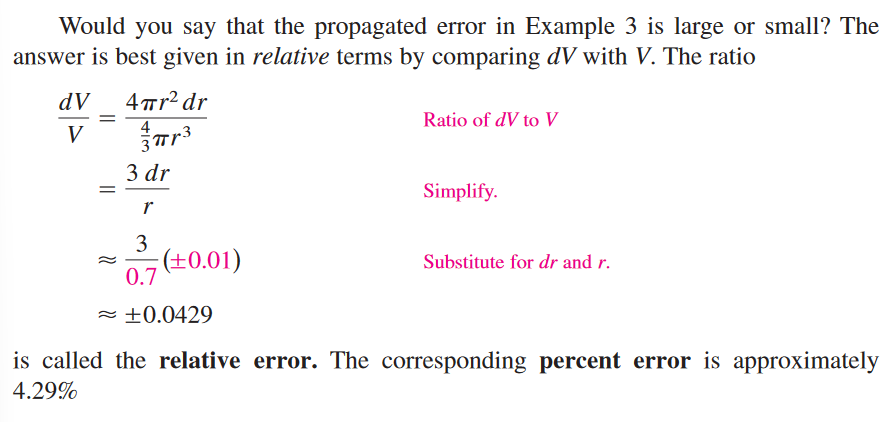
\includegraphics[scale=0.75]{repe.png}












\end{document}